%!TEX root=main.tex
\chapter{Evaluation}
\label{cha:evaluation}

\chapterquote{An ounce of performance is worth pounds of promises.}{Mae West, (1893 - 1980)}

In this chapter, we will investigate the scalability of Gilbert and its performance compared to famous hand-tuned ML algorithms.
We show that Gilbert is not only easily usable in terms of programming but also produces results with decent performance.
Furthermore, we compare the different execution engines and math-backends to see which system gives the best results.
Based on these outcomes, we want to come up with a recommendation for the best configuration of Gilbert.

\section{Experimental Setup}

For our evaluation, we use the $400$-core cluster provided by the DIMA faculty of the Technical University of Berlin.
The cluster comprises $25$ local machines with \SI{32}{\giga\byte} of main memory per computer.
Each machine is equipped with $2$ AMD Opterons 6128 CPUs, each of them having $8$ cores.
The CPUs run at a speed of \SI{2}{\giga\hertz}.

We employ Apache Spark-1.0.0~\cite{spark} for our test runs with the Spark execution engine.
For the Stratosphere execution engine, we use a slightly extended version of Stratosphere-0.6-SNAPSHOT~\cite{stratosphere}.
At the time of evaluation, Stratosphere-0.6 was still under development but we needed the latest features.
Therefore, we use the current snapshot version.
All extensions made to the current snapshot version are also pending pull requests and hopes are high that the final release will contain them all.
Thus, executing Gilbert with the stable release Stratosphere-0.6 should work perfectly fine.
As the underlying distributed file system both systems use Apache Hadoop-1.2.1~\cite{hadoop:2008a}.

The measured execution times on the cluster can slightly differ from measurement to measurement because of non-deterministic factors, such as cache misses, load caused by the operating system and network communication.
In order to cancel out the noise inflicted by these factors, we measure the execution time for each experimental setting five times and report the mean of the measurements.
That way, we reduce the overall variance of the measurements.

\section{Scalability}

The scalability evaluation investigates how Gilbert behaves under increasing work loads and how well it can exploit varying cluster sizes.
As we have implemented Gilbert to provide a scalable linear algebra environment, it is important that it can process data sizes exceeding the main memory of a single machine.
We want to evaluate the scalability performance for Stratosphere's and Spark's execution engine.

\subsection{Matrix Multiplication}
\label{subsec:mm}

As a first benchmark, we choose the matrix multiplication $A\times B$ with $A,B \in \mathbb{R}^{n\times n}$ with $n$ being the dimensionality.
The matrix multiplication operation is demanding, both in CPU load as well as network I/O.
The implementation of the matrix multiplication, shown in \cref{sec:LinearAlgebraOperations}, first joins the column blocks of the left matrix with the row blocks of the right matrix.
This operation replicates the two operands partially and sends them across the network to their respective worker nodes.
For each matching pair of blocks, a local matrix multiplication is executed.
The local matrix multiplication has a complexity of $\mathcal{O}(n_{block}^3)$ with $n_{block}$ being the block size.
The produced intermediate results are grouped according to their left row and right column index.
Finally, the grouped result blocks are added up to give the final result.

The matrices $A$ and $B$ are sparse matrices with uniformly distributed non-zero cells.
They are randomly generated prior to the matrix multiplication, thereby avoiding costly file system I/O.
The sparsity of both matrices is set to $0.001$.
Therefore, both matrices are represented by sparse matrices.
As a baseline, we run the same matrix multiplication on a single machine of the cluster using Gilbert's local execution engine.
The local execution engine uses the same math-backend as the distributed engines and thus serves as a good reference value to see the additional costs of parallel execution.
Breeze is chosen as the math back end for the matrix multiplication.
The Stratosphere and Spark execution engines are both started with \SI{20}{\giga\byte} of main memory for their task managers.
Furthermore, they are both configured to use a similar scheduling strategy, which distributes the work equally among the available computer nodes.
This aspect is especially important in order to compare the results, because some parts of Breeze are multi-threaded and, consequently, take advantage of idling cores.

\subsubsection{Increasing Problem Size}

In the first experiment, we fixed the block sizes to $500 \times 500$ and set the number of cores to $50$.
We then increased the dimensionality $n$ of $A$ and $B$ to observe the runtime behavior.
The resulting execution times for the local, Stratosphere and Spark execution engines are shown in \cref{fig:mmLoadRuntime}.

\begin{figure}[!h]
	\centering
	\begin{subfigure}{\dualpgfwidth}
		\begin{tikzpicture}
			\begin{loglogaxis}[
				xlabel={Dimensionality $n$},
				ylabel={Execution time $t$ in s},
				width=\dualpgfwidth,
				legend entries={Local, Spark, Stratosphere},
				legend pos=north west,
			]
			\addplot[
				color=blue,
				mark=x,
			] table[
				x=RowsA,
				y=Time,
			]
			{data/matrixMultLoad/matrixMultLoadReference};
			\addplot[
				color=red,
				mark=o,
			] table[
				x=RowsA,
				y=Time,
			]
			{data/matrixMultLoad/matrixMultLoadSpark};
			\addplot[
				color=teal,
				mark=triangle,
			] table[
				x=RowsA,
				y=Time,
			]
			{data/matrixMultLoad/matrixMultLoadStratosphere};
			\end{loglogaxis}
		\end{tikzpicture}
		\caption{}
		\label{fig:mmLoadRuntime}
	\end{subfigure}
	\begin{subfigure}{\dualpgfwidth}
		\begin{tikzpicture}
			\begin{semilogxaxis}[
				xlabel={Dimensionality $n$},
				ylabel={Speedup Spark to Stratosphere},
				width=\dualpgfwidth,
				legend pos=north west,
				ymin=0.0,
			]
			\addplot[
				color=red,
				mark=o,
			] table[
				x=RowsA,
				y=Speedup,
			]
			{data/matrixMultLoad/matrixMultLoadSpeedup};
			\end{semilogxaxis}
		\end{tikzpicture}
		\caption{}
		\label{fig:mmSpeedup}
	\end{subfigure}
	\caption{Scalability of matrix multiplication on a $50$-core cluster. \subref{fig:mmLoadRuntime} Execution time of matrix multiplication depending on the data size. \subref{fig:mmSpeedup} Speedup of Spark's execution engine compared to Stratosphere's.}
	\label{fig:mmBenchmark}
\end{figure}

On a single machine, we are able to execute the matrix multiplication for dimensionalities up to $n=10000$ before the system ran out of memory.
We can see that the local execution performs better for dimensionalities $n \le 5000$.
That is expected since the matrix still fits completely in the main memory of a single machine and the distributed execution adds some significant communication overhead.
Furthermore, Spark and Stratosphere both exhibit some noticeable job start up latency which is dominating the execution time for $n\le 10000$.
Those are the reasons why the local executor performs better than the distributed implementations for small matrix sizes.

For matrices with $n>5000$, Spark starts to calculate the matrix multiplication faster than the local executor.
The Stratosphere execution engine does not beat the local computation for sizes which are manageable by a single machine, though.
However, we can observe a steeper ascent of the local execution time compared to Stratosphere.

We also see that Gilbert can handle matrix sizes which scale far beyond the memory capacity of a single machine.
The matrix multiplication for $n=64000$ is finished in \SI{719}{\second} on Spark and in \SI{1230}{\second} on Stratosphere.
We can observe that the Spark execution engine runs consistently faster than Stratosphere.
Since the work load is similar for both systems, the difference has to be caused by the internal functioning of both systems.
For smaller dimensionalities, the execution time of both systems stays almost the same.
Therefore, it has to be mainly caused by the job start up times.
We can consequently infer that Spark is capable of starting its jobs faster than Stratosphere.

Not only does Spark starts its jobs faster, but it also performs better than Stratosphere without exception.
The speedup of Spark's execution engine compared to Stratosphere's execution engine calculating the matrix multiplication is given in \cref{fig:mmSpeedup}.
We can observe that there is a peak speedup of $7$ for $n=2500$.
However, we attribute this value to errors of measurement, because for $n>10000$ the speedup evens out at about $2$ with a slight decrease for $n=64000$.

\subsubsection{Increasing Cluster Size}

In the second experiment, we investigate the scaling behavior of Gilbert with respect to the cluster size.
As a benchmark, we calculate again $A\times B$ with $A,B \in \mathbb{R}^{n\times n}$ and $n$ being the dimensionality.
In order to observe the inflicted communication costs, we keep the work load per core constant while increasing the number of cores.
For this experiment we vary the number of cores from $1$ to $100$ and scale $n$ such that $n^3/\#cores$ is constant.
We started with $n=7500$ for a single core and reached $n=35000$ on $100$ cores.
As block size we chose $500\times 500$.
The results of the experiment are shown in \cref{fig:mmNodesRuntime}.

\begin{figure}[!h]
	\centering
	\begin{tikzpicture}
		\begin{semilogxaxis}[
			xlabel={Number of cores},
			ylabel={Execution time $t$ in s},
			legend pos=north west,
			legend entries={Spark, Stratosphere},
			ymin=0.0,
			ymax=275,
			width=\dualpgfwidth,
		]
		\addplot[
			color=red,
			mark=o,
		] table[
			x=Parallelism,
			y=Time,
		]
		{data/matrixMultCores/matrixMultCoresSpark};
		\addplot[
			color=teal,
			mark=triangle,
		] table[
			x=Parallelism,
			y=Time,
		]
		{data/matrixMultCores/matrixMultCoresStratosphere};
		\end{semilogxaxis}
	\end{tikzpicture}
	\caption{Execution time of matrix multiplication depending on the cluster size with constant work load per core.}
	\label{fig:mmNodesRuntime}
\end{figure}

The optimal scale-out behavior would be a horizontal line.
However, it is impossible to achieve this scale-out behavior due to communication overhead inflicted by parallel execution.
Nonetheless, the results depicted in \cref{fig:mmNodesRuntime} indicate for both execution engines decent scale-out behavior.
Especially for the number of cores $\le 15$, we observe for Stratosphere and Spark an almost horizontal line.
From this point onwards, the scaling of Stratosphere degrades faster than Spark's scaling.
Spark exhibits an outstanding scale-out behavior.
The Spark execution engine requires \SI{90}{\second} to calculate the matrix multiplication with $n=35000$ on $100$ cores.
That is only a slowdown by a factor of $1.5$ if compared to the matrix multiplication with $n=7500$ on a single core, which takes \SI{65}{\second} to finish.
Interestingly, Spark's graph is not monotonic, as one would expect it.
For $\text{\#cores}=50$, we can observe a slight peak in the execution time.
This behavior is counterintuitive.
We suppose that this peculiarity is linked to the internal functioning of the Spark system.

\subsection{Gaussian Non-negative Matrix Factorization}
\label{subsec:NMF}

As second benchmark for evaluating the scalability properties, we choose the Gaussian non-negative matrix factorization (GNMF) algorithm~\cite{seung:anips2001a}.
GNMF finds for a given matrix $V$ a factorization $W$ and $H$ such that $V\approx W H$ holds.
The algorithm is a popular ML algorithm which finds its application in computer vision, document clustering and topic modeling.
In the context of topic modeling, we would have $d$ documents and a set of $w$ words which are contained in the documents.
The goal of topic modeling is to identify the different topics and the words supporting a particular topic.
For this purpose, the matrix $V = (v_{i,j})_{i=1\ldots d,j=1\ldots w}$ is defined, with $v_{i,j}$ containing the frequency of a word $w_j$ appearing in document $d_i$.
By specifying the number of topics $t$, the GNMF algorithm computes $W\in \mathbb{R}^{d\times t}$ and $H\in \mathbb{R}^{t\times w}$ such that $V \approx W H$.
The row $w_i$ of $W$ indicates which topics the document $d_i$ contains and the row $h_i$ of $H$ tells which words correlate with topic $t_i$.
The GNMF algorithm alternately updates the matrices $H$ and $W$ until the result converges.
The algorithm is given in \cref{lst:nmf}.
The operator $.*$, $./$ and $*$ denote the cell wise multiplication, the cell wise division and the matrix multiplication, respectively.

\begin{listing}[!h]
	\begin{CenteredBox}
		\begin{lstlisting}[language=Matlab,
			commentstyle=\color{black},
		  stringstyle=\color{black},
		  keywordstyle=\color{black}\bfseries,
		]
		V = load(); % load matrix to factorize
		W = load(); % load initial values of W
		H = load(); % load initial value of H

		while i < maxIterations
			H = H.*(W'*V ./ W'*W*H); % udpate H
			W = W.*(V*H' ./ W*H*H'); % update W
			i = i + 1;
		end
		\end{lstlisting}
	\end{CenteredBox}
	\caption{Non-negative matrix factorization algorithm.}
	\label{lst:nmf}
\end{listing}

We choose GNMF, because it is a ML algorithm which recently had been implemented for MapReduce systems~\cite{liu:2010a}.
As far as we know, the proposed MapReduce algorithm is one of the best distributed implementations of GNMF.
Thus, it is well suited to assess the performance of Gilbert's implementation of GNMF.

For our evaluation, we calculate one step of the GNMF algorithm.
We set $t=10$, $w=100000$ and vary the number of documents $d$.
The matrix $V\in\mathbb{R}^{d\times 100000}$ is a sparse matrix whose sparsity is set to $0.001$.
The non-zero cells of $V$ are uniformly distributed.
Thus, each line of $V$ contains roughly $100$ non-zero entries, which are drawn from a Gaussian distribution.
The matrices $W$ and $H$ are dense and initialized with random values drawn from a Gaussian distribution.
As a baseline, we run the GNMF on a single machine of the cluster using the local execution engine.
As math back end we choose the Breeze library, which is also used for the distributed execution engines.
Like for the matrix multiplication benchmark, the task manager of Spark and Stratosphere are started with \SI{20}{\giga\byte} of memory and both systems use the same scheduling strategy keeping the work load on all nodes equally distributed.

\subsubsection{Increasing Problem Size}

In the first experiment we fix the number of cores to $50$ and investigate the runtime behavior for increasing values of $d$.
We start with $d=500$ and increase the number of rows of $V$ to $150000$.
The block size of Gilbert is set to $500 \times 500$.
In order to fairly compare the results with the optimized NMF MapReduce implementation proposed in~\cite{liu:2010a}, we re-implemented the algorithm using the Spark and Stratosphere runtime system.
This hand-tuned implementation, henceforth denoted as HT-GNMF, is also executed on $50$ cores.
Additionally, the data is generated having the respective partitioning required by the algorithm.
The execution times of HT-GNMF and Gilbert's GNMF are shown in \cref{fig:nmfLoadRuntime}.

\begin{figure}[!h]
	\centering
	\begin{subfigure}{\dualpgfwidth}
		\begin{tikzpicture}
			\begin{loglogaxis}[
				xlabel={Rows $d$ of $V$},
				ylabel={Execution time $t$ in s},
				width=\dualpgfwidth,
				legend pos=north west,
				legend entries={Local, Spark, Stratosphere, HT-GNMF Spark, HT-GNMF Stratosphere},
				ymax=8000,
			]
			\addplot[
				color=blue,
				mark=x,
			] table[
				x=Rows,
				y=Time,
			]
			{data/nnmfStepLoad/nnmfStepLoadReference};
			
			\addplot[
				color=red,
				mark=o,
			] table[
				x=Rows,
				y=Time,
			]
			{data/nnmfStepLoad/nnmfStepLoadSpark};
			
			\addplot[
				color=teal,
				mark=triangle,
			]table[
				x=Rows,
				y=Time,
			]
			{data/nnmfStepLoad/nnmfStepLoadStratosphere};
			\addplot[
				color=black,
				mark=diamond,
			]table[
				x=rowsV,
				y=time,
			]
			{data/nnmfStepLoad/gnmfStepLoadSpark};
			\addplot[
				color=magenta,
				mark=square,
			]table[
				x=rowsV,
				y=time,
			]
			{data/nnmfStepLoad/gnmfLoadStratosphere};
			\end{loglogaxis}
		\end{tikzpicture}
		\caption{}
		\label{fig:nmfLoadRuntime}
	\end{subfigure}
	\begin{subfigure}{\dualpgfwidth}
		\begin{tikzpicture}
			\begin{semilogxaxis}[
				xlabel={Rows $d$ of $V$},
				ylabel={Speedup of HT-GNMF on Spark},
				width=\dualpgfwidth,
				ymin=0,
				legend entries={Spark,Stratosphere},
				legend pos=north west,
			]
			\addplot[
				color=red,
				mark=o,
			] table[
				x=Rows,
				y=Speedup,
			]
			{data/nnmfStepLoad/gnmfStepLoadSpeedupSpark};

			\addplot[
				color=teal,
				mark=diamond,
			] table[
				x=Rows,
				y=Speedup,
			]
			{data/nnmfStepLoad/gnmfStepLoadSpeedupStratosphere};
			\end{semilogxaxis}
		\end{tikzpicture}
		\caption{}
		\label{fig:gnmfSpeedup}
	\end{subfigure}
	\caption{Scalability of GNMF on a $50$-core cluster. \subref{fig:nmfLoadRuntime} Execution time of one GNMF step depending on the data size. \subref{fig:gnmfSpeedup} Speedup of HT-GNMF running on Spark compared to Gilbert's GNMF using the Spark and Stratosphere execution engine, respectively.}
	\label{fig:nmfBenchmark}
\end{figure}

The local executor can be applied to sizes of $d$ ranging from $500$ to $1500$ rows, before the data exceeded the available main memory of a single computer.
As expected, the local execution performs far better for these data sizes than the distributed execution with Stratosphere.
However, the GNMF and the HT-GNMF executed on Spark outperformed the local execution.
That is rather surprisingly, since the distributed execution should inflict some noticeable communication overhead.
But apparently the parallelism compensates for the additional communication costs.

The distributed systems can also be used for data sizes which exceed the memory of a single computer.
Both distributed execution engines scale well up to the point where Spark and Stratosphere can no longer keep the data in memory.
The two data flow systems have to perform internal sorting, partitioning and shuffling steps to implement the high level operations, such as join, reduce, cogroup and cross.
If the memory size is not sufficient to execute these steps, then the data will be gracefully spilled to disk.
On the one hand, this behavior makes the systems more robust and applicable to data sizes which largely exceed the total amount of memory.
But on the other hand, the performance abruptly deteriorates massively once the data has to be spilled.
For the Stratosphere and Spark executor, we experienced this behavior for $d>50000$ and $d>150000$, respectively.
For data sizes bigger than these thresholds, the benchmark runs became so slow that we could not finish them and discarded these runs as infeasible.

For Stratosphere, this behavior ensues earlier due to its specific memory management.
Stratosphere assigns each cluster node a specific number of slots.
The default value is the number of cores.
The memory is then split evenly among the slots.
Once the task managers have started and assigned the memory to each slot, it is not possible to dynamically transfer memory portions between slots.
Therefore, the effectively available memory for each task is considerably smaller than the initial \SI{20}{\giga\byte}.
Additionally, Stratosphere's ability to support streaming further decreases the per task memory.
Currently, it is assumed that all tasks belonging to one pipeline can be deployed simultaneously to one slot.
In order to execute all pipeline tasks, the slot memory will be further divided by the number of tasks which can be concurrently run.

In contrast to that, Spark separates the execution of different operations into distinct stages.
A stage is only submitted for execution, after all preceding stages have been completed.
That way, the memory does not have to be splitted between succeeding tasks and thus spilling occurs later.

The runtime of HT-GNMF running on Spark, the Stratosphere and the Spark executor differ for varying data sizes almost by a constant factor.
The fastest implementation for $d\le 100000$ is the HT-GNMF algorithm running on Spark.
The speedup of HT-GNMF running on Spark compared to GNMF on Spark's and Stratosphere's executor is shown in \cref{fig:gnmfSpeedup}.
It can be seen that HT-GNMF runs approximately $1.7$ times faster than Gilbert's GNMF using the Spark executor.
Compared to the Stratosphere execution engine, we can observe that HT-GNMF runs faster and faster for increasing $d$.
HT-GNMF achieves a speedup of approximately $16$ for $d=50000$.
The different runtime behaviors of Spark's and Stratosphere's execution engines are most likely caused by the Spark and Stratosphere system, since the linear algebra operations are implemented identically.
The runtime behavior of HT-GNMF running on Stratosphere is interesting.
At first, it performs rather poorly compared to its Spark counterpart.
However, for $d>100000$ it suddenly outperforms the Spark implementation.
Thus, GNMF scales better if it is executed on Stratosphere. 

Even though, Gilbert can not even reach the performance of HT-GNMF, the development using Gilbert was considerably easier.
One GNMF step can be programmed in five lines of Gilbert code, whereas we needed $28$ lines of Scala code for Spark's HT-GNMF and $70$ lines of Scala code for Stratosphere's HT-GNMF.
Not only did we have to know how to program Spark and Stratosphere, but it also took us quite some time to verify the correct functioning of both implementations.
The verification was made significantly more difficult and time-consuming due to a programming bug we introduced.
The debugging process showed us quite plainly how tedious the development process even with systems like Spark and Stratosphere can be.
Thus, the productivity increase gained by using a high-level declarative programming language for linear algebra must not be neglected and compensates for the performance loss.
\Textcite{alvaro:2010a} made a similar observations while developing a declarative programming language for distributed systems programming.

\subsubsection{Increasing Cluster Size}

In the second experiment of the GNMF benchmark, we analyze how Gilbert scales-out when increasing the cluster size while keeping the work load for each core constant.
We vary the cluster size from $1$ core to $100$ cores and scale the number of documents $d$ accordingly.
Initially we start with $1000$ documents and, consequently, calculate the matrix factorization for $100000$ documents on $100$ cores.
The ideal behavior would be a horizontal line.
However, this outcome cannot be expected, since the GNMF computation requires communication between the cluster nodes.
The results of this experiment are shown in \cref{fig:nmfNodesRuntime}.

\begin{figure}[h!]
	\centering
	\begin{tikzpicture}
			\begin{semilogxaxis}[
				xlabel={Number of cores},
				ylabel={Execution time $t$ in s},
				ymin=0,
				legend entries={Spark, Stratosphere},
				legend pos=north west,
				width=\dualpgfwidth,
			]
			\addplot[
				color=red,
				mark=o,
			] table[
				x=Parallelism,
				y=Time,
			]
			{data/nnmfStepCores/nnmfStepCoresSpark};

			\addplot[
				color=teal,
				mark=diamond,
			] table[
				x=Parallelism,
				y=Time,
			]
			{data/nnmfStepCores/nnmfStepCoresStratosphere};
			\end{semilogxaxis}
		\end{tikzpicture}
		\caption{Execution time of one GNMF step depending on the cluster size with constant work load per core.}
		\label{fig:nmfNodesRuntime}
\end{figure}

The scale-out behavior of the Stratosphere and Spark execution engines both show good results for $\#cores \le 5$.
For higher degrees of parallelism, Stratosphere's performance quickly deteriorates.
On $50$ cores, Stratosphere needs \SI{1082}{\second}, whereas Spark needs only \SI{113}{\second}.
We could not finish Stratosphere's computations for higher degrees of parallelism than $50$, because the system simply became too slow.
That vast performance decline is most likely caused by data spilling at some internal operation.
In contrast to Stratosphere, Spark does not suffer from these limitations for the number of cores we tested.
In fact, it almost exhibits an extraordinary scale-out behavior with an almost constant runtime.
The runtime on $100$ cores is only two times slower than the runtime on a single core with the same work load per core.

\section{Block Size}

The block size has a significant influence on the overall performance of Gilbert since it directly controls the data parallelism and data granularity of the local operations.
The bigger the block size is, the fewer blocks are available for parallel computations.
But the bigger the block size is, the more work can be done on a single computer without having to communicate with other nodes.
To measure the effect of the block size on the performance, we calculate a single GNMF step with varying block sizes using the Spark execution engine.
For this benchmark we set $d=100000$, $w = 100000$ and $t = 10$.
The remaining parameters are set like in \cref{subsec:NMF}.
The execution times for different block sizes are shown in \cref{fig:blocksizesNMFStep}.

\begin{figure}
	\centering
	\begin{subfigure}[t]{\dualpgfwidth}
		\begin{tikzpicture}
			\begin{axis}[
				ymin=0,
				ylabel={Execution time $t$ in s},
				width=\dualpgfwidth,
				ybar,
				xtick={0,1,2,3,4,5},
				xticklabels={
				25 x 25,
				50 x 50,
				100 x 100,
				500 x 500,
				1000 x 1000,
				2000 x 2000
				},
				x tick label style={rotate=45,anchor=east, /pgf/number format/1000 sep=},
				height=159pt,
			]
			\addplot[
				color=blue,
				fill=blue,
			]table[
				x=Idx,
				y=Time,
			]
			{data/nnmfStepBlocksizes/nnmfStepBlocksizesSpark100000};
			\end{axis}
		\end{tikzpicture}
		\caption{}
		\label{fig:blocksizesNMFStep}
	\end{subfigure}
	\begin{subfigure}[t]{\dualpgfwidth}
		\begin{tikzpicture}
			\begin{loglogaxis}[
				xlabel={Rows $d$ of $V$},
				ylabel={Execution time $t$ in s},
				width=\dualpgfwidth,
				legend entries = {25 x 25, 500 x 500, 1000 x 1000},
				legend pos=north west,
			]
			\addplot[blue,
				mark=x,
			] table[
				x=Rows,
				y=Time,
			]
			{data/nnmfStepBlocksize/nnmfStepBlocksize25Spark};

			\addplot[red,
				mark=o,
			] table[
				x=Rows,
				y=Time,
			]
			{data/nnmfStepBlocksize/nnmfStepBlocksize500Spark};

			\addplot[teal,
				mark=diamond,
			] table[
				x=Rows,
				y=Time,
			]
			{data/nnmfStepBlocksize/nnmfStepBlocksize1000Spark};
			\end{loglogaxis}
		\end{tikzpicture}
		\caption{}
		\label{fig:nmfStepDifferentBlocksizes}
	\end{subfigure}
	\caption{Execution time of a single GNMF step for different block and input sizes using Spark's execution engine on a $50$-core cluster. \subref{fig:blocksizesNMFStep} Execution time of a single GNMF step with constant input depending on the block size. \subref{fig:nmfStepDifferentBlocksizes} Execution time of a single GNMF step depending on the number of rows for different block sizes.}
	\label{fig:blocksizes}
\end{figure}

The graph shows that we have a minimal runtime for a block size of $500 \times 500$.
Apparently, this block size constitutes the best trade-off between data parallelism and data granularity.
For lower block sizes, the additional overhead introduced by indexing information and the low data granularity increases the runtime.
For higher block sizes, the decreased parallelism devours the benefits of a high data granularity.
That evaluation justifies our block size choice of $500 \times 500$.

The effect of different block sizes is also compared in \cref{fig:nmfStepDifferentBlocksizes} where we computed one GNMF step with the Spark execution engine for varying sizes of $V$.
The GNMF algorithm is executed on $50$ cores of the cluster using the Breeze math back end.
We can observe that we obtain better results with an increased block size.
Clearly, the block size $25 \times 25$ is inferior to the block sizes $500\times 500$ and $1000\times 1000$.
However, the results between the last two block sizes do not differ in a significant way.

It is important to stress that there is no single block size, which is optimal for all problems and all computer architectures.
The best degree of parallelism and the best data granularity strongly depends on the problem, its inputs and the used computing machine.
Therefore, it is not possible to specify an ideal block size, which, instead, should be determined for each task individually.

\section{Optimization}

In this section, we want to evaluate the effects Gilbert's optimizer has on the runtime of programs.
For this purpose, we execute one GNMF step on Gilbert's Stratosphere and Spark execution engine using the same settings as in \cref{subsec:NMF}.
However, this time we disable the transpose pushdown and matrix-multiplication reordering optimization.
The results are shown in \cref{fig:nnmfLoadOptimization}.

\begin{figure}
	\centering
	\begin{subfigure}[t]{\dualpgfwidth}
		\begin{tikzpicture}
			\begin{semilogxaxis}[
				xlabel={Rows $d$ of $V$},
				ylabel={Execution time $t$ in s},
				legend pos=north west,
				legend entries={Optimized Spark, Optimized Stratosphere, Non-optimized Spark, Non-optimized Stratosphere},
				width=\dualpgfwidth,
			]
			
			\addplot[
				color=red,
				mark=o,
			] table[
				x=Rows,
				y=Time,
			]
			{data/nnmfStepLoadNoOp/nnmfStepLoadSpark};
			
			\addplot[
				color=teal,
				mark=triangle,
			]table[
				x=Rows,
				y=Time,
			]
			{data/nnmfStepLoadNoOp/nnmfStepLoadStratosphere};

			\addplot[
				color=blue,
				mark=x,
			] table[
				x=Rows,
				y=Time,
			]
			{data/nnmfStepLoadNoOp/nnmfStepNoOpLoadSpark};

			\addplot[
				color=black,
				mark=diamond,
			]table[
				x=Rows,
				y=Time,
			]
			{data/nnmfStepLoadNoOp/nnmfStepNoOpLoadStratosphere};
			
			\end{semilogxaxis}
		\end{tikzpicture}
		\caption{}
		\label{fig:nnmfLoadOptimization}	
	\end{subfigure}
	\begin{subfigure}[t]{\dualpgfwidth}
		\begin{tikzpicture}
			\begin{semilogxaxis}[
				xlabel={Rows $d$ of $V$},
				ylabel={Speedup},
				legend pos=north west,
				legend entries={Optimized Spark, Optimized Stratosphere},
				width=\dualpgfwidth,
			]
			
			\addplot[
				color=red,
				mark=o,
			] table[
				x=Rows,
				y=Speedup,
			]
			{data/nnmfStepLoadNoOp/gnmfStepLoadSpeedupSpark};
			
			\addplot[
				color=teal,
				mark=triangle,
			]table[
				x=Rows,
				y=Speedup,
			]
			{data/nnmfStepLoadNoOp/gnmfStepLoadSpeedupStratosphere};			
			\end{semilogxaxis}
		\end{tikzpicture}
		\caption{}
		\label{fig:gnmfLoadOptimizationSpeedup}
	\end{subfigure}
	\caption{Effect of Gilbert's optimizations using the example of a single GNMF step executed on a $50$-core cluster. \subref{fig:nnmfLoadOptimization} Execution time of the optimized and non-optimized GNMF step depending on the input size. \subref{fig:gnmfLoadOptimizationSpeedup} Speedup of the optimized GNMF step with respect to the non-optimized GNMF step depending on the input size.}
\end{figure}

We can observe that the Gilbert optimizer has a significant effect on the runtime of GNMF.
The optimized Gilbert program runs on both distributed engines faster than it's non-optimized counterparts.
Interestingly, the Spark execution engine seems to benefit more from the optimizer than the Stratosphere executor.
The speedups of the optimized GNMF step with respect to its non-optimized counterparts are shown in \cref{fig:gnmfLoadOptimizationSpeedup}
For the optimized program running on Spark's execution engine, a steadily ascending speedup, except for $d=500$, can be observed.
The optimized Spark version runs about $18$ times faster than the non-optimized program for $d=10000$.
In contrast to that, Stratosphere shows a constant speed-up of roughly $1.7$ between the optimized and non-optimized version.

It is not yet known what causes these different speed-ups.
However, looking at the NMF formula in \cref{lst:nmf}, we can explain why the optimization works.
There are two matrix multiplications which can be optimized: $W^T WH$ in line $6$ and $WHH^T$ in line $7$.
Keeping in mind that $W\in \mathbb{R}^{d\times 10}$ and $H\in \mathbb{R}^{10 \times 100000}$, we can assess the different strategies.
The non-optimized version would execute the matrix multiplications due to left-associativity from left to right:

\begin{displaymath}
	\overbrace{\underbrace{\left(W^T W\right)}_{\in \mathbb{R}^{10\times 10}}H}^{\in\mathbb{R}^{10\times 100000}}
\end{displaymath}

and

\begin{displaymath}
	\overbrace{\underbrace{\left(WH\right)}_{\in \mathbb{R}^{d \times 100000}}H^T}^{\in \mathbb{R}^{d\times 10}}
\end{displaymath}

For the first matrix multiplication, the execution order is optimal, since the intermediate result of $W^T W$ is much smaller than $WH$.
However, for the second matrix multiplication, the execution order is far from optimal.
The left-associativity produces an intermediate matrix result of size $d\times 100000$.
For large $d$ this matrix becomes really huge.
Additionally, the intermediate result is dense, because the operands $W$ and $H$ are dense, as well.
By changing the execution order, we can decrease the size of the intermediate result significantly.

\begin{displaymath}
	\overbrace{W\underbrace{\left(HH^T\right)}_{\in \mathbb{R}^{10 \times 10}}}^{\in \mathbb{R}^{d\times 10}}
\end{displaymath}

The Gilbert optimizer first detects the matrix multiplication reordering and then changes it so that the maximum intermediate result is minimized.
That is the reason why the optimized GNMF program runs clearly faster.

\section{Gilbert Algorithms vs. Specialized Algorithms}

In this section, we want to investigate how well algorithms implemented in Gilbert perform compared to specialized algorithms.
We expect that the Gilbert runtime adds some overhead as trade-off for their easy-to-use programming interface.
Furthermore, the high-level linear algebra abstraction of Gilbert might make it difficult to exploit certain properties to speed up the processing.
Therefore, we believe that the hand-tuned algorithms will get the upper hand.

For our comparison, we chose two famous ML algorithms, which can be expressed in terms of linear algebra: PageRank and \kmeans.
Since both algorithms are iterative, we can demonstrate Gilbert's loop support.
We first execute them directly in Gilbert, given the Gilbert code, and then run them directly on Stratosphere and Spark.
For the direct execution, we have implemented both algorithms using the Stratosphere and Spark API.
In contrast to Gilbert, the direct implementation requires a deep understanding of the underlying runtime system.
Furthermore, the distributed implementation is far from trivial compared to the linear algebra representation of the original problem.

\subsection{PageRank}

The PageRank algorithm~\cite{page:1999a} is the famous algorithm developed by Larry Page and Sergey Brin to compute a ranking between any kind of entities with reciprocal quotations and references.
Initially, it was developed to rank the web sites of the world wide web, which it did so well that Google grew quickly into a multi-billion dollar company.
PageRank is only one algorithm comprising Google's web search, but it is probably one of the best known.

\subsubsection{Algorithm}

The idea of PageRank is to estimate the rank of a web site based on the ranks of other web sites, which link to this site.
It is assumed that high quality web sites are more likely to link to other high quality web sites.
Thus, these sites get a high rank with which they can ``vote'' for other sites.

The PageRank can also be explained by the model of a ``random'' surfer.
Assume there is a surfer which randomly follows an outgoing link from a web site.
Occasionally, or if he ends up in a dead end, the surfer enters a random URL in his address bar.
That way, he will eventually visit the whole web.
By tracking the time he spends on each web site, an importance measure for each site is obtained.
Web sites, which are linked by pages on which the random surfer spends more time, will receive more clicks by the random surfer and thus a higher importance.
That importance measure is in fact the PageRank.

Even though the problem seems to be self-referencing, the PageRank vector turns out to be the solution to an eigenvalue problem.
Thus, the PageRank vector can be easily computed using a power iteration.
PageRank's MATLAB code is given in \cref{lst:PageRankVanilla}.

\begin{listing}[!h]
	\begin{CenteredBox}
		\begin{lstlisting}[language=Matlab,
		commentstyle=\color{black},
		  stringstyle=\color{black},
		  keywordstyle=\color{black}\bfseries,
		  morekeywords={ones},]
% load adjacency matrix
A = load(); 
maxIterations = 10;
d = sum(A, 2); % outdegree per vertex
% create the column-stochastic transition matrix
T = (diag(1 ./ d) * A)'; 
r = ones(numVertices, 1) / numVertices; % initialize the ranks
e = ones(numVertices, 1) / numVertices;
% PageRank calculation
while i < maxIterations
	r = .85 * T * r + .15 * e
	i = i + 1
end
		\end{lstlisting}
	\end{CenteredBox}
	\caption{MATLAB PageRank implementation.}
	\label{lst:PageRankVanilla}
\end{listing}

The power iteration happens in the while loop, where the PageRank vector $r$ is iteratively multiplied with the transition matrix $T$.
In order to execute this code with Gilbert, the while loop has to be replaced with a fixpoint operation.
As it can be seen in \cref{lst:gilbertPageRank}, the replacement is only of syntactic nature.

\begin{listing}[!h]
	\begin{CenteredBox}
		\begin{lstlisting}[language=Matlab,
		commentstyle=\color{black},
		  stringstyle=\color{black},
		  keywordstyle=\color{black}\bfseries,
		  morekeywords={ones, fixpoint},]
% load adjacency matrix
A = load();
maxIterations = 10;
d = sum(A, 2); % outdegree per vertex
% create the column-stochastic transition matrix
T = (diag(1 ./ d) * A)'; 
r_0 = ones(numVertices, 1) / numVertices; % initialize the ranks
e = ones(numVertices, 1) / numVertices;
% PageRank calculation
fixpoint(r_0, @(r) .85 * T * r + .15 * e, maxIterations)
		\end{lstlisting}
	\end{CenteredBox}
	\caption{Gilbert PageRank implementation.}
	\label{lst:gilbertPageRank}
\end{listing}

A common implementation of PageRank for Spark and Stratosphere works as follows.
The PageRank vector is represented by a set of tuples $(w_i, r_i)$ with $w_i$ denoting the web site $i$ and $r_i$ being its rank.
The adjacency matrix is stored row-wise as a set of tuples $(w_i, A_i)$ with $w_i$ denoting the web site $i$ and $A_i$ being its adjacency list.
For the adjacency list $A_i$, it holds that $w_j \in A_i$ if and only if there exists a link from web site $i$ to $j$.

Given the PageRank vector and the adjacency matrix representation, the next PageRank vector can be computed the following way.
At first, the PageRank $r_i$ of web site $i$ is joined with its adjacency list $A_i$.
For each outgoing link $w_j \in A_i$ a new tuple $(w_j, 0.85r_i/\left|A_i\right|)$ with the rank of $i$ being divided by the number of outgoing links is created.
In order to incorporate the random jump behavior to any available web site, a tuple $(w_i, 0.15/|w|)$, with $|w|$ being the number of all web sites, is generated for each web site $i$.
In order to compute the next PageRank vector, all newly generated tuples are grouped according to their ID.
The resulting groups are reduced by adding up all partial rank values.
This calculation produces the new PageRank vector.
By executing these steps iteratively, the PageRank algorithm is obtained.
One step of the PageRank algorithm is depicted as a data flow plan in \cref{fig:pageRankDataFlow}.

\begin{figure}[!h]
	\centering
	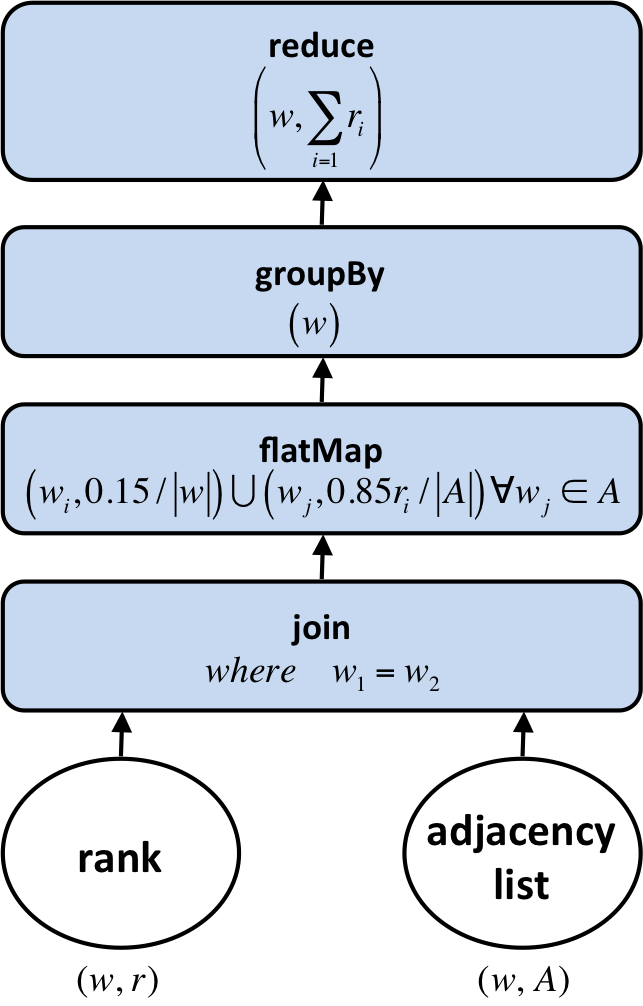
\includegraphics[width=.3\linewidth]{images/pageRankStep.png}
	\caption{Data flow of one iteration of the PageRank algorithm for Spark and Stratosphere.}
	\label{fig:pageRankDataFlow}
\end{figure}

\subsubsection{Experiment}

For comparison, $10$ steps of the PageRank algorithm for varying sizes of the adjacency matrix $A$ are calculated.
The adjacency matrix $A$ is a sparse matrix of size $n \times n$ with a sparsity of $0.001$.
For each test run, the matrix is randomly generated so that their non-zero cell entries are uniformly distributed.
The computation is executed on $50$ cores of the DIMA cluster.
The block size is set to $500 \times 500$ and Breeze is chosen as math back end for Gilbert's distributed execution engines.
The execution times are depicted in \cref{fig:pageRankResults}.

\begin{figure}
	\centering
	\begin{subfigure}[h]{\dualpgfwidth}
		\begin{tikzpicture}
			\begin{loglogaxis}[
				xlabel={Number of vertices $n$},
				ylabel={Execution time $t$ in s},
				legend pos=north west,
				legend entries={Gilbert Spark, Gilbert Stratosphere, Specialized Stratosphere,Specialized Spark},
				width=\dualpgfwidth,
			]
			
			\addplot[blue,
				mark=x,
			] table[
				x=NumVertices,
				y=Time,
			]
			{data/pagerank/pagerankSpark};

			\addplot[red,
				mark=o,
			] table[
				x=NumVertices,
				y=Time,
			]
			{data/pagerank/pagerankStratosphere};

			\addplot[teal,
				mark=diamond,
			] table[
				x=rows,
				y=time,
			]
			{data/pagerank/pagerankBenchStratosphere};

			\addplot[black,
				mark=triangle,
			] table[
				x=rows,
				y=time,
			]
			{data/pagerank/pagerankBenchSpark};
			\end{loglogaxis}
		\end{tikzpicture}
		\caption{}
		\label{fig:pageRankResults}
	\end{subfigure}
	\begin{subfigure}[h]{\dualpgfwidth}
		\begin{tikzpicture}
			\begin{semilogxaxis}[
				xlabel={Number of vertices $n$},
				ylabel={Speedup},
				legend pos=north west,
				legend entries={Specialized Spark, Specialized Stratosphere},
				width=\dualpgfwidth,
			]
			
			\addplot[blue,
				mark=x,
			] table[
				x=NumVertices,
				y=Speedup,
			]
			{data/pagerank/pagerankSpeedupSpark};

			\addplot[red,
				mark=o,
			] table[
				x=NumVertices,
				y=Speedup,
			]
			{data/pagerank/pagerankSpeedupStratosphere};
			\end{semilogxaxis}
		\end{tikzpicture}
		\caption{}
		\label{fig:pageRankSpeedup}
	\end{subfigure}
	\caption{Comparison of Gilbert's PageRank implementation with specialized algorithms on Spark and Stratosphere running on $50$-core cluster. \subref{fig:pageRankResults} Execution time of $10$ steps of the PageRank algorithm depending on the adjacency matrix's size. \subref{fig:pageRankSpeedup} Speedup of specialized algorithms with respect to Gilbert's implementations.}
	\label{fig:pageRankEvaluation}
\end{figure}

The graph shows that the directly implemented PageRank algorithm runs clearly faster than Gilbert's versions of PageRank.
For Stratosphere, we were only able to compute Gilbert's PageRank for $50000$ web sites, before the computation became too slow to execute.
Even though Spark's execution engine showed a similar runtime behavior for $25000 \le n \le 50000$, Spark was able to scale up to $n=100000$.

The specialized algorithms show a better scalability.
For both systems, Spark and Stratosphere, we could compute the PageRank for up to $150000$ web sites.
Interestingly, the Stratosphere system scales better for the specialized algorithm than Spark.
For $n\ge 25000$, Stratosphere shows significant faster execution times.
It is not yet fully clear what causes this difference.
We assume that the fault tolerance mechanism of Spark is responsible for the performance loss.
With increasing number of iterations and data size, Spark also has to increase the lineage information stored for a possible data recovery.
This lineage information costs CPU time and consumes memory.
Since it is not possible to disable the fault-tolerance mechanism, one has to keep this aspect in mind when comparing Stratosphere with Spark.

The speedup of the specialized algorithms with respect to Gilbert's implementations for this experiment is shown in \cref{fig:pageRankSpeedup}.
For $n\le 25000$, the hand-tuned algorithms running on Spark and Stratosphere show a similarly increasing speedup.
The Stratosphere and Spark version achieve a speedup of approximately $14$ and $10$ for $n=50000$, respectively.
For $n\ge 50000$ Spark seems to exhibit a constant speedup.

The performance difference between the specialized algorithm and Gilbert's version can be explained by considering the different execution plans.
As shown in \cref{fig:pageRankDataFlow}, each iteration of the specialized PageRank algorithm comprises one join, one group reduce and one flat map operation.
The flat map operation can be executed without communication between the nodes.
The join and reduce operation requires the data to be sent over the network.
Thus, most of the time should be spent executing the join and reduce operation.

Looking at line $10$ of \cref{lst:gilbertPageRank}, it can be seen that one matrix-vector product, two vector-scalar products and one vector sum have to be computed for each iteration of Gilbert's PageRank algorithm.
Remembering \cref{sec:LinearAlgebraOperations}, we can deduce that all these operations require two cross, two join and one reduce operation.
The two cross operations, where one of the operands is a scalar value, can be realized efficiently by simply broadcasting this value.
However, the two join operations and the reduce operation require to shuffle the available data and thus inflict some serious network communication costs.

Comparing the specialized algorithm with Gilbert's implementation, it can be clearly seen that the high-level linear algebra representation adds three additional operations, with one of them being highly expensive.
Therefore, it is not surprising that the specialized PageRank algorithm performs better.

\subsection{\kmeans}

The \kmeans clustering algorithm~\cite{macqueen:1967a} is very popular for cluster analysis in data mining.
The goal of \kmeans is to partition the available $n$ data points into $k$ clusters, where each data point is assigned to the cluster with the nearest mean.
Even though the optimal solution is NP-hard, heuristic algorithms exist to compute approximations.

\subsubsection{Algorithm}

The standard algorithm alternately assigns the data points to its nearest intermediate cluster and calculates new intermediate cluster centers as the mean of all assigned data points.
The initial cluster centers are usually randomly selected points from the set of data points or random points.
The MATLAB code for the \kmeans algorithm, shown in \cref{lst:kmeansMatlab}, is a little bit cumbersome if one wants to write it down in matrix notation.

\begin{listing}
	\begin{CenteredBox}
		\begin{lstlisting}[language=Matlab,
		commentstyle=\color{black},
		  stringstyle=\color{black},
		  keywordstyle=\color{black}\bfseries,
		  morekeywords={pdist2, repmat, },]
datapoints = load();
centers = load();
mask = repmat((1:numCenters), numDatapoints, 1)';
for i = 1:maxIterations
		distances = pdist2(datapoints, centers);
		assignments = min(distances, [], 2);
		repIdx = repmat(assignments', numCenters, 1);
		multiplier = repIdx == mask;
		divisor = repmat(sum(multiplier, 2), 1, dimension);
		centers = (multiplier*datapoints)./divisor;
end
		\end{lstlisting}
	\end{CenteredBox}
	\caption{MATLAB \kmeans implementation.}
	\label{lst:kmeansMatlab}
\end{listing}

The data points and centers are stored row-wise in the matrices \code{datapoints} and \code{centers}.
The first step, assigning each data point to its nearest center, is done in the lines $5$ and $6$.
The \code{pdist2} function calculates the pairwise euclidean distance between the rows of its two operands, in this case, the current centers and the data points.
Once all pairwise distances have been calculated, the nearest cluster center is selected for each data point.
This computation is done in line $6$.
The \code{assignments} column vector contains the index of the nearest cluster center for each data point.
In order to calculate the new cluster centers as the mean of all assigned data points, some repmat magic has to be introduced.
The idea is to construct for each center a logical row vector which indicates all data points assigned to this cluster.
The computation is achieved by generating a matrix which contains in each row the \code{assignments} vector.
The matrix has as many rows as there are clusters.
The generated matrix is compared with \code{mask} in line $8$, whose cells are set to the row index of the cell.
That gives the aforementioned indicator matrix.
By adding the entries of each row, the number of data points assigned to a cluster center can be computed.
The new cluster centers and thus the second step of the algorithm are obtained as the result of a matrix multiplication and cellwise matrix division in line $10$.	

Compared to the MATLAB representation, the direct implementation for Spark and Stratosphere seems rather simple.
The first difference is that the data points are represented as tuples of the form $(id_i, p_i)$ with $id_i$ being the identifier of data point $i$ and $p_i$ being its coordinates.
The clusters are represented likewise as tuples $(id_j, c_j)$ with $c_j$ being the coordinates of the cluster center.
In order to calculate the pairwise distances between the data points $p_i$ and the clusters $c_j$, the Cartesian product of the two datasets is constructed.
This operation produces all combinations of data point cluster pairs.
Having the coordinates of the data point and the cluster center, the distance can easily be computed.
The output of the distance computation is a tuple of the form $(id_i, p_i, id_j, \norm{p_i - c_j}_2)$, the data point ID, the data point coordinates, the cluster center ID and the distance.
The cluster center with the minimal distance can be selected by grouping on the data point id $id_i$ and selecting the cluster center ID with minimal distance. 
The result of the reduce operation has the form $(id_j, p_i)$ with $id_j$ being the nearest cluster center ID.
In order to calculate the new cluster centers, the current data set has to be grouped on the cluster center ID.
The generated groups contain the data points, which are assigned to the respective cluster center. 
The new cluster centers are computed by adding all data points $p_i$ of each group up and dividing the result by the number of points contained in the groups.
These operations constitute a single iteration step.
The \kmeans algorithm is obtained by repeating the iteration step until the cluster centers converge.
The dataflow plan of a single iteration step is depicted in \cref{fig:kmeansDataflow}.

\begin{figure}
	\centering
	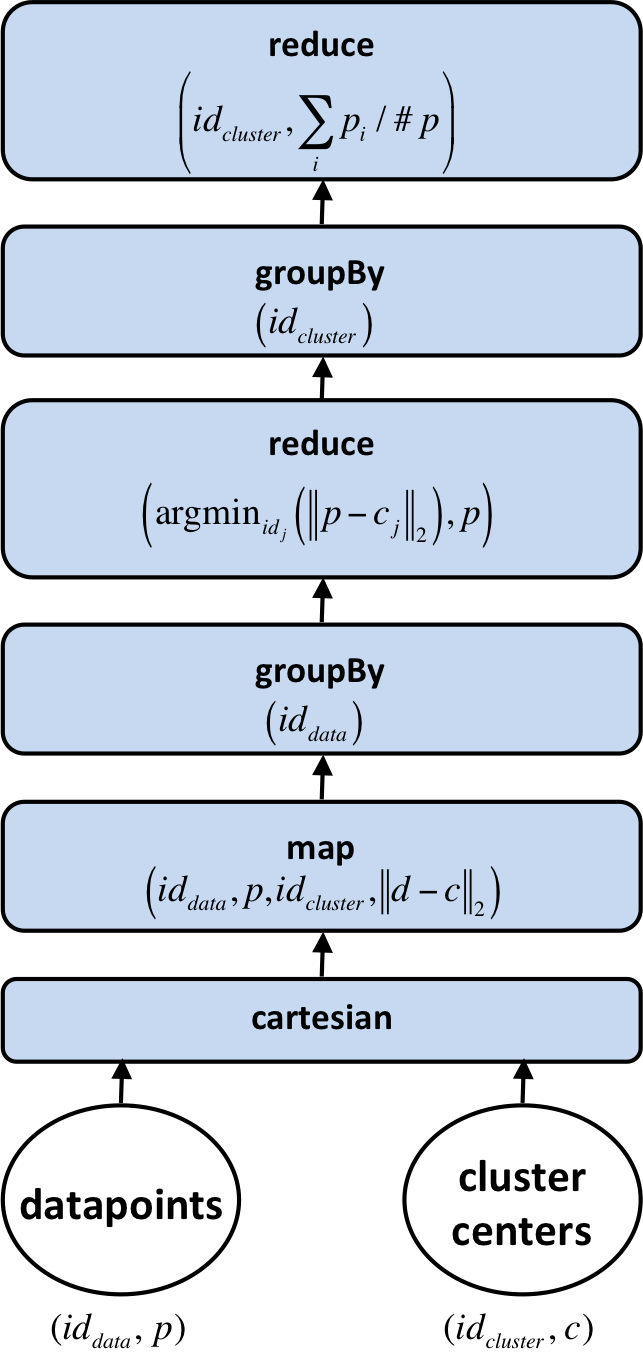
\includegraphics[width=0.3\linewidth]{images/kmeansStep.png}
	\caption{Dataflow plan of a single \kmeans step.}
	\label{fig:kmeansDataflow}
\end{figure}

The execution time of Gilbert's \kmeans implementation is compared with the execution time of the hand-tuned algorithms.
The Gilbert code is given in \cref{lst:kmeansGilbert}.
As it can be seen, the only differences between the MATLAB and Gilbert version are the \code{fixpoint}, the \code{linspace} and the \code{minWithIndex} function.
The \code{linspace} function generates a linearly spaced row vector, as it is known from MATLAB.
The \code{minWithIndex} function returns the minimum value of the specified dimension and its index as column vectors in a cell array.

\begin{listing}
	\begin{CenteredBox}
		\begin{lstlisting}[language=Matlab,
		commentstyle=\color{black},
		  stringstyle=\color{black},
		  keywordstyle=\color{black}\bfseries,
		  morekeywords={repmat, pdist2, minWithIndex, fixpoint}
		  ]
datapoints = load();
centers = load();
mask = repmat(linspace(1, numCenters, numCenters), ...
	numDatapoints, 1)';
function newCenters = kmeansStep(centers)
		distances = pdist2(datapoints, centers);
  	assignments = minWithIndex(distances, 2);
  	repIdx = repmat(assignments{2}', numCenters, 1);
  	multiplier = repIdx == mask;
  	divisor = repmat(sum(multiplier, 2), 1, dimension);
  	newCenters = (multiplier*datapoints)./divisor;
end
fixpoint(centers,@kmeansStep, maxIterations)
		\end{lstlisting}
	\end{CenteredBox}
	\caption{Gilbert \kmeans implementation.}
	\label{lst:kmeansGilbert}
\end{listing}

\subsubsection{Experiment}

For the experiments, $10$ steps of the \kmeans algorithms on the $50$-core DIMA cluster are calculated.
The algorithms compute $100$ cluster centers from $n$ data points.
The points are $2$-dimensional.
The number of data points is varied from $1000$ to $1000000$.
The data points and the initial cluster centers are drawn from a uniform distribution.
The block size is set to $500\times 500$.
The results of the experiment are depicted in \cref{fig:kmeansResult}.

\begin{figure}
	\centering
	\begin{subfigure}[h]{\dualpgfwidth}
		\begin{tikzpicture}
			\begin{loglogaxis}[
				xlabel={Number of data points $n$},
				ymax=5000,
				ylabel={Execution time $t$ in s},
				legend pos=north west,
				legend entries={Gilbert Spark, Gilbert Stratosphere, Specialized Stratosphere},
				width=\dualpgfwidth,
			]
			
			\addplot[blue,
				mark=x,
			] table[
				x=NumDatapoints,
				y=Time,
			]
			{data/kmeans/kmeansSpark};

			\addplot[red,
				mark=o,
			] table[
				x=NumDatapoints,
				y=Time,
			]
			{data/kmeans/kmeansStratosphere};

			\addplot[teal,
				mark=diamond,
			] table[
				x=numDatapoints,
				y=time,
			]
			{data/kmeans/kmeansBenchStratosphere};
			\end{loglogaxis}
		\end{tikzpicture}
		\caption{}
		\label{fig:kmeansResult}
	\end{subfigure}
	\begin{subfigure}[h]{\dualpgfwidth}
		\begin{tikzpicture}
			\begin{semilogxaxis}[
				xlabel={Number of data points $n$},
				ylabel={Speedup},
				legend pos=north west,
				legend entries={Specialized Stratosphere},
				width=\dualpgfwidth,
				ymin=0,
			]
			
			\addplot[red,
				mark=o,
			] table[
				x=NumDatapoints,
				y=Speedup,
			]
			{data/kmeans/kmeansSpeedupStratosphere};
			\end{semilogxaxis}
		\end{tikzpicture}
		\caption{}
		\label{fig:kmeansSpeedup}
	\end{subfigure}
	\caption{Comparison of Gilbert's \kmeans with specialized algorithm on Stratosphere. \subref{fig:kmeansResult} Execution time of $10$ steps of the \kmeans algorithm on $50$-cores depending on the adjacency matrix's size. \subref{fig:kmeansSpeedup} Speedup of specialized algorithm with respect to Gilbert's implementation.}
	\label{fig:kmeansBenchmark}
\end{figure}

We observe that Gilbert's \kmeans implementations perform more slowly than the specialized implementation.
We could only calculate $100000$ points with Gilbert, because the computation took too long to finish for more points.
The speedup of the specialized algorithm with respect to Stratosphere's execution engine is shown in \cref{fig:kmeansSpeedup}.
With an increasing number of data points $n$, the speedup increases monotonically.
For $n=100000$ the specialized implementation achieves a speed-up of $8$ and $10$ compared to the Spark executor and Stratosphere executor, respectively.
Thus, we can conclude that the specialized algorithm of \kmeans executing on Stratosphere not only runs faster but also scales better than Gilbert's implementations.
Interestingly, we were not able to run the specialized algorithm on Spark because the two reduce operations caused the system to become unbearably slow.

If we take a closer look at the execution plans of both algorithms, it becomes clear why Gilbert performs so poorly.
For each step of the specialized algorithm, the dataflow system has to execute one Cartesian, one map and two group reduce operations.
The two group reduce and the Cartesian operation are responsible for most of the work load, because they cause significant network I/O.

For Gilbert, the execution plan is more complex.
Looking at the iteration step in \cref{lst:kmeansGilbert}, the following summation is obtained:
The \code{pdist2} function is implemented using one join, one map and one group reduce operation.
The \code{minWithIndex} function uses three Cartesian, one group reduce and two cogroup operations.
The \code{repmat} function comprises three Cartesian and one cogroup operation.
The comparison operator in line $9$ requires one join operation.
The matrix multiplication and cellwise matrix division in line $11$ is implemented using two join and one reduce operation.
In total, one step of Gilbert's \kmeans algorithm inflicts four join, nine Cartesian, four cogroup and three group reduce operations.
Consequently, it can be concluded that the linear algebra abstraction of Gilbert comes at the price of a more complex and thus longer running execution plan.

\section{Breeze vs. Mahout Math-Backend}

As we have explained in \cref{sec:mathBackend}, Gilbert supports two math back ends for the computation of local tasks.
The principal math back end uses the Breeze library for high performance linear algebra operations.
As an alternative, Gilbert also supports the popular Mahout math library.

As first benchmark, the matrix multiplication from \cref{subsec:mm} is repeated with the Mahout library.
The benchmark calculates the matrix multiplication of two sparse matrices $A,B\in\mathbb{R}^{n\times n}$ with $n$ being their dimensionality.
The matrices have a sparsity of $0.001$.
The computation is executed on $50$ cores and we use a block size of $500\times 500$.
The results are given in \cref{subfig:mmMathBackend}.

\begin{figure}
	\centering
	\begin{subfigure}{\dualpgfwidth}
		\begin{tikzpicture}
			\begin{semilogxaxis}[
				xlabel={Dimensionality $n$},
				ylabel={Execution time $t$ in s},
				legend pos=north west,
				legend entries={Breeze Spark, Breeze Stratosphere, Mahout Spark, Mahout Stratosphere},
				width=\dualpgfwidth,
				xtick=data,
				log ticks with fixed point,
			]
			
			\addplot[
				color=red,
				mark=o,
			] table[
				x=RowsA,
				y=Time,
			]
			{data/matrixMultLoad/matrixMultBreezeLoadSpark};
			
			\addplot[
				color=teal,
				mark=triangle,
			]table[
				x=RowsA,
				y=Time,
			]
			{data/matrixMultLoad/matrixMultBreezeLoadStratosphere};

			\addplot[
				color=blue,
				mark=x,
			] table[
				x=RowsA,
				y=Time,
			]
			{data/matrixMultLoad/matrixMultMahoutLoadSpark};

			\addplot[
				color=black,
				mark=diamond,
			]table[
				x=RowsA,
				y=Time,
			]
			{data/matrixMultLoad/matrixMultMahoutLoadStratosphere};
			
			\end{semilogxaxis}
		\end{tikzpicture}
		\caption{}
		\label{subfig:mmMathBackend}
	\end{subfigure}
	\begin{subfigure}{\dualpgfwidth}
		\begin{tikzpicture}
			\begin{semilogxaxis}[
				xlabel={Rows $d$ of $V$},
				ylabel={Execution time $t$ in s},
				legend pos=north west,
				legend entries={Breeze Spark, Breeze Stratosphere, Mahout Spark, Mahout Stratosphere},
				width=\dualpgfwidth,
			]
			
			\addplot[
				color=red,
				mark=o,
			] table[
				x=Rows,
				y=Time,
			]
			{data/nnmfStepLoad/nnmfStepBreezeLoadSpark};
			
			\addplot[
				color=teal,
				mark=triangle,
			]table[
				x=Rows,
				y=Time,
			]
			{data/nnmfStepLoad/nnmfStepBreezeLoadStratosphere};

			\addplot[
				color=blue,
				mark=x,
			] table[
				x=Rows,
				y=Time,
			]
			{data/nnmfStepLoad/nnmfStepMahoutLoadSpark};

			\addplot[
				color=black,
				mark=diamond,
			]table[
				x=Rows,
				y=Time,
			]
			{data/nnmfStepLoad/nnmfStepMahoutLoadStratosphere};
			
			\end{semilogxaxis}
		\end{tikzpicture}
		\caption{}
		\label{subfig:nmfMathBackend}
	\end{subfigure}
	\caption{Comparison of Breeze and Mahout math back end. \subref{subfig:mmMathBackend} Runtime of matrix multiplication on $50$-core cluster depending on the dimensionality $n$ using Breeze and Mahout. \subref{subfig:nmfMathBackend} Runtime of single GNMF step on $50$-core cluster depending on the number of rows $d$ of $V$ using Breeze and Mahout.}
	\label{fig:nnmfLoadMathBackend}
\end{figure}

The results of the matrix multiplication demonstrate impressively that Breeze is far superior to Mahout in multiplying two sparse matrices.
Even for relatively small matrix sizes, the execution times differ strikingly.
For $n=2500$, Spark's and Stratosphere's execution engine using the Mahout library take \SI{723}{\second} and \SI{745}{\second} to finish the computation, respectively.
By contrast, the same computation using the Breeze library finishes after \SI{10}{\second} and \SI{71}{\second} on Spark and Stratosphere, respectively.
The performance gap even widens for an increasing dimensionality $n$.
For $n=5000$, Breeze reaches a speed-up of $100$ compared to Mahout.
It can be concluded that even for relatively small matrix sizes the multiplication using Mahout takes so long that it can hardly be regarded feasible.

The mystery of this bad performance can be unraveled by taking a look into the source code of Mahout.
Mahout offers a sparse matrix implementation, based on hash maps.
However, it does not provide an efficient algorithm for this data structure.
Instead, Mahout uses the standard matrix multiplication algorithm.
Thus, for each resulting element $c_{i,j}$, Mahout iterates over the complete row $a_i$ of $A$ and column $b^{j}$ of $B$, even though most of the row and column entries will be zero.
Even worse, each access triggers an hash map look up.
In total, the matrix multiplication has to perform $2n^3$ hash table look ups and $n^3$ hash table insertions.

In contrast to Mahout, Breeze implements the sparse matrix using the compressed sparse column (CSC) storing scheme, which stores the data in a continuous array.
This approach not only avoids costly hash map look ups, but Breeze also implements an optimized matrix multiplication algorithm for CSC.
The algorithm is aware of the sparse nature of its operands and accesses only elements which are non-zero in both matrices.

As second benchmark, we repeated the GNMF computation from \cref{subsec:NMF}.
We calculated a single GNMF step for varying number of rows $d$ of $V$ on $50$-cores of our cluster.
The number of rows $d$ reaches from $500$ to $10000$.
As before, the sparsity of $V$ is $0.001$ and its non-zero cells are distributed uniformly.
The sizes of $W$ and $H$ are $d\times 10$ and $10 \times 100000$, respectively.
For the benchmark, we set the block size to $500 \times 500$.
The runtimes of the Breeze and Mahout math back end are given in \cref{subfig:nmfMathBackend}.

It can be clearly seen that GNMF runs faster with Breeze as math back end on the Stratosphere as well as on the Spark execution engine.
On Spark, Breeze reaches a speed-up of roughly $4$ for $d=10000$. 
On Stratosphere, Breeze reaches a speed-up of about $1.75$ for the same number of rows.

We can conclude that Breeze has a better support for sparse matrix operations.
Breeze also performs better for operations on mixed sparse and dense matrices as it is the case for GNMF.
However, the gap is not as striking as it is the case for sparse matrix operations only.
In conclusion, we highly recommend using Breeze as the math back end in order to experience best performance with Gilbert programs.

